\section{Entorno de Desarrollo Local}

Para garantizar la reproducibilidad del proyecto, en esta sección se descibirá el entrono de desarrollo en el que se ha realizado y el acceso al repositorio con el código fuente.

\subsection{Tecnologías y Versiones}

El proyecto se ha desarrollado en un entorno \textbf{Windows 10}, aunque esto no influye en la compatibilidad, ya que todas las tecnologías utilizadas son multiplataforma, lo cual permite realizar el desarrollo en cualquier sistema operativo sin restricciones. En la tabla \ref{tab:dependencias_versiones} se presentan las tecnologías principales empleadas en el proyecto junto con sus versiones correspondientes.

\begin{table}[htbp]
    \centering
    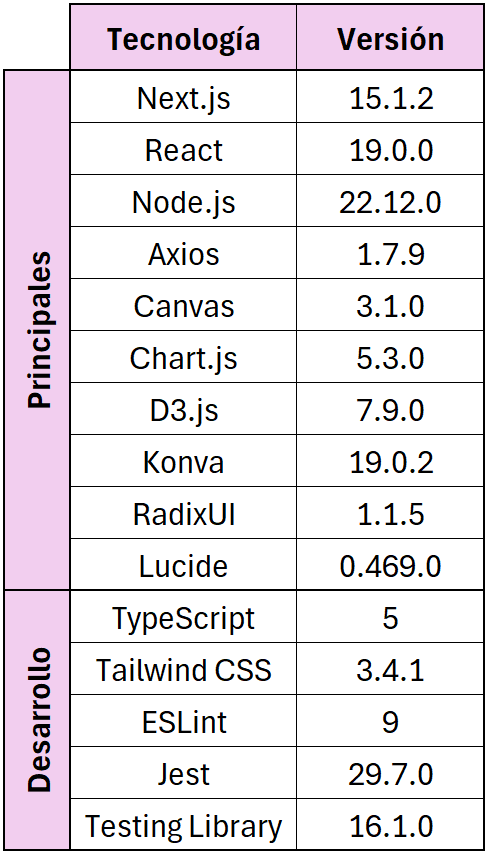
\includegraphics[width=0.37\textwidth]{figures/dependencias_versiones.png}
    \captionsetup{skip=5pt}
    \caption{Dependencias usadas en el desarrollo, junto con sus versiones.}
    \label{tab:dependencias_versiones}
\end{table}

Cabe destacar que el gestor de paquetes utilizado en el proyecto ha sido \textbf{\texttt{pnpm} (\textit{Performant Node Package Manager})}, en lugar de \texttt{npm} (\textit{Node Package Manager}) o \texttt{yarn} (\textit{Yet Another Resource Negotiator}). La elección de \texttt{pnpm} se debe a sus mejoras en la gestión de dependencias y optimización del uso del espacio de almacenamiento. A diferencia de \texttt{npm}, \texttt{pnpm} utiliza un sistema de enlaces en lugar de duplicar archivos en cada proyecto, lo que reduce significativamente el consumo de espacio. Además, \texttt{pnpm} es completamente compatible con los paquetes del registro de \texttt{npm}, lo que garantiza su interoperabilidad con la mayoría de los ecosistemas de desarrollo basados en \textit{Node.js}.

\subsection{Instalación y Configuración del Proyecto}

El proyecto se encuentra alojado en un repositorio de \textit{GitHub}\footnote{Repositorio del proyecto: \href{https://github.com/jonortega/tfg-app-spotify}{https://github.com/jonortega/tfg-app-spotify}} para evitar pérdidas y tener disponibilidad completa al código. Para ejecutarlo localmente, además de haber instalado \textit{Node.js}, hay que clonar el respositorio, acceder a la carpeta y ejecutar los comandos de instalación y ejecución. A continuación, se muestran los comandos necesarios para realizar estos pasos:

\begin{ifalgorithm}[H]
    \begin{lstlisting}[language=bash]
    # Clonar el repositorio
    git clone https://github.com/jonortega/tfg-app-spotify.git
    
    # Acceder al directorio del proyecto
    cd tfg-app-spotify
    
    # Instalar dependencias
    pnpm install
    
    # Ejecutar el servidor de desarrollo
    pnpm run dev
    \end{lstlisting}
    \caption{Comandos de instalación y ejecución inicial del proyecto.}
    \label{alg:instalacion_proyecto}
\end{ifalgorithm}

Tras estos pasos, la página web estará accesible en \texttt{localhost:3000}. Es encesario agregar un fichero de variables de entorno \texttt{.env.local}, ya que, por seguridad, no se registra en el sistema de control de versiones. El contenido de dicho fichero se muestra en el \hyperref[ch:anexoC]{Anexo C} (algoritmo \ref{alg:variables_entorno}).

Dos de las variables de entorno necesarias para poder tratar con la API de \textit{Spotify}, son el \textbf{Client ID} y el \textbf{Client Secret}. Estos dos valores se obtienen al realizar el registro de la aplicación en la plataforma de desarrollo de \textit{Spotify}. En la siguiente sección, se explicará cómo realizar este registro y dónde obtener dichas variables.

\newpage

\section{Registro de la Aplicación en Spotify}

Para poder obtener datos de la Web API de \textit{Spotify}, es necesario registra la aplicación en su plataforma de desarrollo\footnote{Spotify for Developers: \href{https://developer.spotify.com/}{https://developer.spotify.com/}}. Tras inciar con una cuenta, se nos presentará un panel donde podremos crear una nueva app. \textit{Spotify} pedirá algunos datos (figura \ref{fig:create_app}), que tendremos que rellenar. Los campos como \textit{Redirect URIs} pueden ser modificados posteriormente, ya que tendremos que actualizarlo con el dominio indicado tras el despliegue de la aplicación.

\begin{figure}[H]
    \centering
    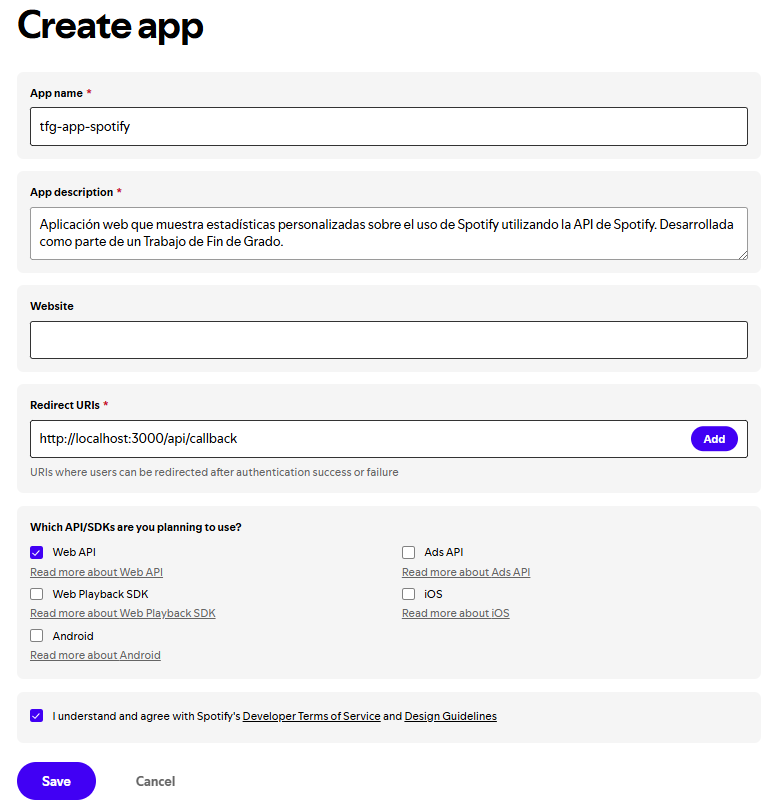
\includegraphics[width=0.65\textwidth]{figures/registro_spotify/create_app.png}
    \caption{Panel de creación de app en la plataforma de \textit{Spotify}.}
    \label{fig:create_app}
\end{figure}

Al aceptar los términos y crear la app, tendremos acceso al \textit{Client ID} y \textit{Client Secret}. Estos se encuentran en los ajustes (\textit{settings}) y tendremos que expandir el panel para poder ver los dos valores (figura \ref{fig:client_id_secret}).

\begin{figure}[H]
    \centering
    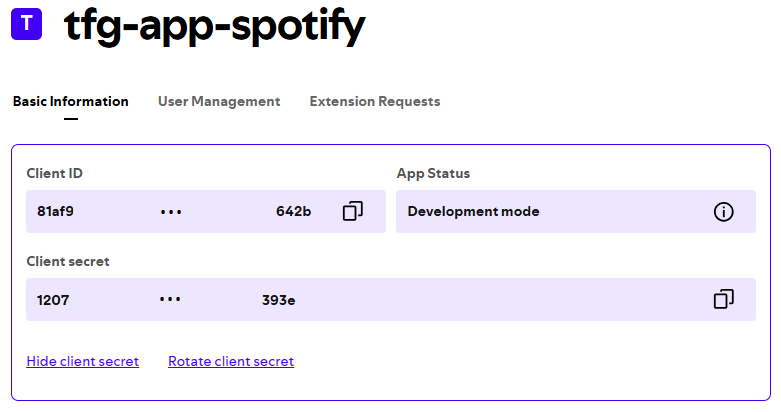
\includegraphics[width=0.65\textwidth]{figures/registro_spotify/client_id_secret.png}
    \caption{Panel de ajustes con el \textit{Client ID} y el \textit{Client Secret}.}
    \label{fig:client_id_secret}
\end{figure}

En el caso en el que el \textit{Client Secret} haya sido comprometido, es posible generar uno nuevo, anulando el anterior y evitando tener que desechar la aplicación registrada. También se muestra un campo llamado \textit{App Status} con el valor \textbf{Development Mode}. Esto significa que la aplicación registrada está en ``desarrollo'', por lo que existen las siguientes restricciones:

\begin{itemize}
    \item Un máximo de 25 usuarios (cuentas verificadas de \textit{Spotify}) pueden usar la aplicación.
    \item Cada usuario tiene que estar registrado en una lista de permitidos (\textit{allowlist}) de la plataforma.
\end{itemize}

Es posible eliminar estas restricciones, enviando una solicitud a \textit{Spotify} para cambiar el estado de \textit{Development Mode} a \textbf{Extended Quota Mode}. En el caso de que sea aceptada, se elimina cualquier restricción sobre el número de usuarios permitidos y no será necesario registrarlos anteriormente, además de ampliar el umbral de la tasa de peticiones (\textit{rate limit}). En este trabajo \textbf{no se va a realizar dicha solicitud}, por lo que tendremos que acogernos a las limitaciones impuestas en el modo de desarrollo. Esto requiere que se registren las cuentas de usuarios que vayan a probar la aplicación en la pestaña de gestión de usuarios (figura \ref{fig:user_management}).

\begin{figure}[H]
    \centering
    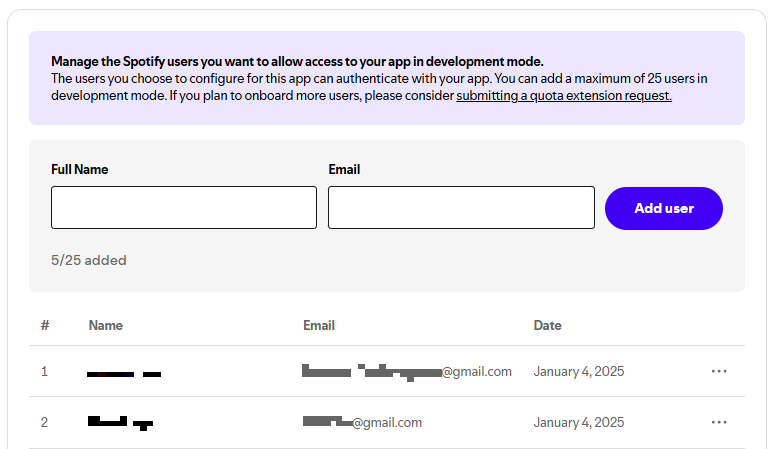
\includegraphics[width=0.75\textwidth]{figures/registro_spotify/user_management.png}
    \caption{Panel de gestión de usuarios que tienen acceso a la aplicación.}
    \label{fig:user_management}
\end{figure}

Con estos pasos, se habrá realizado correctamente el registro de la aplicación y obtención del \textit{Client ID/Secret}, imprescindibles para la comunicación con la API de \textit{Spotify}. En la plataforma de desarrollo, además, tenemos accesible un panel para poder monitorear la actividad de la aplicación (\hyperref[ch:anexoC]{Anexo C}, figura \ref{fig:dashboard_spotify}).

\section{Ciclo de Desarrollo}

El ciclo de desarrollo del proyecto ha seguido un enfoque híbrido entre los modelos \textbf{incremental} e \textbf{iterativo}. En concreto, se ha construido en tres incrementos, realizados en diferentes puntos del proyecto. En cada uno, se han añadido más funcionalidades (incremental) y refinando las ya existentes (iterativo). A continuación se describe cada incremento con más detalle.

\subsection*{Incremento I: Prototipado Rápido}

Durante la fase inical de adquisición de competencias, se desarrolló un prototipo rápido para validar la viabilidad técnica del proyecto. No se buscaba crear la base desde donde seguir trabajando una vez inicase el desarrollo formal; si no que, utilizando herramientas más simples, se quería obtener una idea preliminar de cómo se podrían implementar las funcionalidades principales. No se utilizaron las tecnologías finales del desarrollo, por lo que gran parte del código implementado no fue reutilizado.

En este prototipo se implementaron las siguientes funcionalidades, en diferentes grados de completado:
\setlength{\itemsep}{0pt}
\begin{itemize}
    \item Inicio de sesión de un usuario y obtención de los tokens.
    \item Renovación del \texttt{access\_token} mediante el \texttt{refresh\_token}.
    \item Obtener los \textit{top items} del usuario.
    \item Obtener las canciones favoritas del usuario.
    \item Obtener los \textit{track features} (\textbf{no implementado en el producto final}).
    \item Prototipos de las estadísticas:
          \begin{itemize}
              \item \textit{Hall Of fame}
              \item \textit{Huella Del Día}
              \item \textit{La Bitácora}
          \end{itemize}
\end{itemize}

\subsection*{Incremento II: Producto Mínimo Viable (PMV)}

Una vez terminada la planificación del proyecto, se dio comienzo a una primera implementación del sistema, desarrollando una base de código que formaría parte del producto final. En esta fase, se utilizaron todas las tecnologías finales seleccionadas para el desarrollo, incluyendo \textit{Next.js}, \textit{React}, TypeScript y \textit{Tailwind CSS}.

Durante este incremento, se completaron las siguientes partes fundamentales del sistema:

\setlength{\itemsep}{0pt}
\begin{itemize}
    \item Estructura completa de páginas de la aplicación web.
    \item Implementación de los endpoints mediante \textit{Route Handlers}.
    \item Inicio de sesión y cierre de sesión seguros.
    \item Gestión segura de los tokens.
    \item Implementación de las estadísticas básicas \textit{Top Tracks}, \textit{Top Artists}, \textit{Top Genres} y \textit{Recently Played}.
    \item Desarrollo inicial de las seis estadísticas avanzadas finales en un estado funcional básico.
\end{itemize}

Si bien estas estadísticas se implementaron de manera inicial y sin refinamientos, su propósito principal fue definir la interacción entre el frontend y el backend, establecer los tipos de datos y endpoints exactos requeridos, y detectar posibles problemas en la presentación de la información. Asimismo, esta fase permitió identificar la necesidad de herramientas adicionales, como bibliotecas de gráficos, en caso de que las opciones disponibles no fueran suficientes.

En términos generales, este incremento sirvió para caracterizar con mayor precisión el alcance del proyecto y definir con claridad los aspectos que deberían considerarse en las siguientes etapas de análisis y diseño. A diferencia del prototipo inicial, gran parte del código desarrollado en esta iteración se integró directamente en la versión final del sistema.

\subsection*{Incremento III: Producto Final}

Finalmente, en el último incremento se completaron todas las funcionalidades secundarias pendientes, junto con una serie de optimizaciones de rendimiento, ajustes en las estadísticas avanzadas y mejoras en la interfaz y experiencia de usuario. Esta fase marcó la consolidación del sistema y la preparación del código para su despliegue.

Las principales funcionalidades implementadas y correcciones realizadas fueron:

\setlength{\itemsep}{0pt}
\begin{itemize}
    \item Posibilidad de cambiar el rango temporal en los módulos \textit{Top Tracks}, \textit{Top Artists} y \textit{Top Genres}.
    \item Implementación de la funcionalidad para crear playlists en \textit{Hall Of Fame}.
    \item Desarrollo de la estadística \textit{Tus Décadas} utilizando la librería \textit{Konva} para una mayor optimización.
    \item Mejora en la presentación y rendimiento de la estadística \textit{Índice de Interferencia} con \textit{D3.js}.
    \item Corrección en la estructura de datos enviada desde el backend a la estadística \textit{La Bitácora}.
    \item Implementación de la ventana informativa sobre la \textit{Política de Privacidad}.
    \item Reemplazo de la implementación manual de la ventana modal de las estadísticas por la librería \textit{Radix UI}.
    \item Creación de componentes de carga (\textit{loading components}).
    \item Gestión de errores encontrados al probar con diferentes cuentas de usuario.
    \item Desarrollo de una pantalla de carga específica para las estadísticas avanzadas.
    \item Refactorización del código para crear funciones reutilizables, como en la obtención de datos (\textit{fetch}), facilitando la gestión de los componentes.
    \item Preparación del código para su despliegue en \textit{Vercel}, especialmente la gestión de variables de entorno.
\end{itemize}

Este último incremento permitió completar todas las funcionalidades planeadas y refinar el sistema en su conjunto. Además de las mejoras implementadas, se documentaron posibles optimizaciones futuras, aunque, dentro del alcance definido para el proyecto, la aplicación alcanzó un estado final funcional y estable.

Cabe destacar que las listas de funcionalidades y mejoras descritas en cada incremento no son exhaustivas, sino que recogen las implementaciones y cambios más relevantes realizados durante el desarrollo. A lo largo del proceso, se llevaron a cabo numerosas correcciones, ajustes e implementaciones adicionales que no se han detallado en su totalidad. No obstante, estas listas permiten ofrecer una visión general de los aspectos más significativos de cada incremento en el desarrollo del proyecto.

\section{Implementación del Fronted}

\subsection{Lógica de las Estadísticas}

\subsection{React Hooks}

\section{Implementación del Backend}

\subsection{Lógica y Tratamiento de Datos en el Servidor}

\subsection{Estructuras de Datos}

\section{Optimizaciones}